\chapter{Probing the Small Scale Structure of Galactic Magnetic field}
%title tbd
\label{ch: RMsynth}

This chapter describes the work additional to the source finding that I have carried out in order to be able to run the 1-dimensional polarimetry pipeline on the data cube EMU1505-60, and then details the running of the pipeline's processes. When complete, the POSSUM science ready processing pipeline will conduct all the steps discussed in this chapter as well as making a correction for the ionospheric Faraday rotation and mosaic together adjacent fields of observation. As I am only processing one observation field, the ionospheric Faraday rotation is a few rad$\,$m$^{\shortminus2}$ and is constant across the field, so it would not affect the results of the structure function analysis detailed within this chapter. 

\section{Pre-Pipeline Processing}

\subsection{Convolution}

Before I ran the pipeline on the Stokes cubes I smoothed the I, Q and U cubes to a common resolution across all channels. This means that further analysis which is affected by resolution is easier to carry out. The Stokes data cubes all have 288 channels representing differing frequencies within the observation band. Each data cube was resampled to get three pixels across the final beam size and all maps were convolved using the CONVL task within AIPS. The cubes were then remade using the MCUBE task.

\subsection{Noise Profile}

My next step was to find the background noise of the image so that the I could accurately assign a weighting to each frequency channel to favour the least noisy channels. To do this, I first used AIPS to find the coordinates of five boxes which I made to contain as few sources as possible by selecting boxes manually within predominantly empty regions of the observed field. These boxes are shown in Figure \ref{fig: background noise boxes}.

\begin{figure}
    \centering
    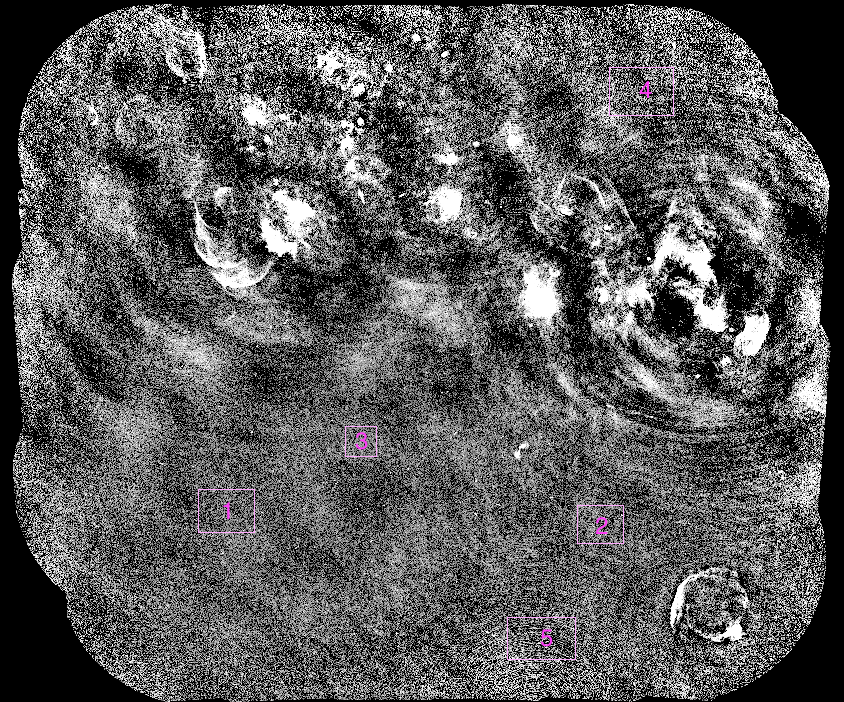
\includegraphics[width=0.9\linewidth]{Thesis_Template/Figures/Boxes for noise calculation image.png}
    \caption{Boxes chosen for background noise calculations}
    \label{fig: background noise boxes}
\end{figure}

I created smaller cubes of all frequency channels for each box, combined the boxes by stacking them into a single matrix and found the standard deviation of each frequency channel across all five boxes, which was very low between the different noise backgrounds ($<0.0004$). These are the values used in the pipeline for the weighting of the frequency channels.


\section{POSSUM Polarimetry Pipeline}
\label{POSSUM pipeline 1d}
The POSSUM polarimetry pipeline is the pipeline that will be applied to all the POSSUM fields in order to achieve one of the collaboration's core science case of producing an RM grid that covers the entire southern sky (\cite{POSSUM}). It mainly uses software from the RM-tools package created by \cite{RMtools} \footnote{RM-tools can be accessed at https://github.com/CIRADA-Tools/RM-Tools/tree/master}. This pipeline currently has two main routes: the 1-dimensional pipeline and the 3-dimensional pipeline. 


The 1D pipeline produces Faraday rotation measurements for sources in the predefined catalogue. From this pipeline I used eight steps: read sourcelist, extract spectra, diffuse subtraction, save spectra, rm synth 1D, clean catalog, write catalog and save FDFs.

The first step, read sourcelist, takes the output catalogue created by the source finding algorithm in the form of a fits file and turns it into an astropy table of dictionaries for each source. As the source finder used by ASKAP is Selavy, the pipeline was written to accommodate the format of the Selavy output catalogue. As I instead used PyBDSF as the source finder, I needed to change the names of the variables and conversion factors in order to account for the difference in input. Apart from this step, I ran each step as it had been written, my only input being selecting options and specifying input parameters.

The next step extracts the Stoke I, Q and U spectrum for each source in the source list and the median spectra for the diffuse emission surrounding the source. This is done by taking the mean pixel intensity for each source and the median and noise of the annulus around the source, with the inner and outer radii of the annulus given in the configuration file. The mean intensity is calculated by finding the sum of a 3x3 and 5x5 pixel window centred on the nearest listed source, in order to capture the slightly the off-peak polarisation and finally the sum is normalised using the synthesised Gaussian beam model. This method was found to be an improvement on the method of using the peak pixel as it is less sensitive to variations of the true source position within the peak pixel. The noise of the annulus is determined by applying an annulus shaped mask at each frequency for the source and taking the standard deviation. The annulus chosen had an inner radius of 35'' and an outer radius of 109''. This size means that it is possible that other sources could be in it, so this method of averaging over all frequency bands helps to negate their influence on the noise. The pipeline stores these as a dictionary. Any sources that are too close to the image edge are noted in the log file and their spectra assigned zero values. This was the case for 118 of the 3860 sources found by the source finding routine. The next step, diffuse subtraction, subtracts the median, from the annulus, from each source spectrum calculated in the previous step. These spectra are saved, so that they can be used again without re-extraction. This is useful because the extract spectra step takes over an hour to complete.

The next step is rotation measure synthesis, which for the one dimensional pipeline performs RM synthesis along single lines of sight using RM-tools. 
This routine uses a discrete Fourier transform to calculate the Faraday dispersion function (FDF) using the equation to transform the spectra from frequency space to Faraday depth space. In order to achieve RM synthesis a FDF is fit to each spectrum, using Equation \ref{eq: discrete rm synth}. The formal Fourier inversion of complex Faraday dispersion function

\begin{equation}
    F(\phi)=\frac{1}{\pi}\int^{+\infty}_{\shortminus\infty}P(\lambda^2)e^{\shortminus2i\phi\lambda^2}d\lambda^2
    \label{eq: inverse of FDF}
\end{equation}

\noindent cannot itself be used to reconstruct the FDF from Equation \ref{eq: complex FDF} because it is not possible to measure polarisation emission at negative wavelengths or to observe polarisation emission at all wavelengths, especially crucial wavelengths close to zero \cite{Li_2011}. Therefore a digitised and weighted version must be used such as Equation \ref{eq: discrete rm synth}. 





The weighting of the data was chosen to be inverse variance in order to down weight noisy channels. This process weights each channel by the inverse variance, which is ideally proportional to the frequency width, whereas Equation \ref{eq: inverse of FDF} weights by interval of $\lambda^2$. Given $\lambda = \frac{c}{\nu}$, $|d\lambda^2| = 2c^2\frac{1}{\nu^3}d\nu$, which means that summing over $d\nu$ in the real integral would put a factor of $\nu^3$ into the weight. In practice, however, this does not affect POSSUM's RMSF (Equation \ref{eq: RMSF}) as $\nu$ only varies $\pm 15 \%$ around the central wavelength and comparison of the two weightings shows no significant difference.


The width of a $sinc(\theta)$ function, such as in the RMSF function, $R(\phi)$ (Equation \ref{eq: RMSF}), is measured as $\delta\theta = 3.79$ between half power points, so the width of $R(\phi)$, and thus the maximum Faraday depth is 

\begin{equation}
    \delta\phi \approx \frac{3.79}{\Delta\lambda^2}
    \label{}
\end{equation}


\noindent (e.g. \cite{Dickey_2019}). The Faraday depth sampling limit is half that of the equation above:

\begin{equation}
    ||\phi_{max}|| \approx \frac{1.9}{\delta\lambda^2}
    \label{eq: sampling limit}
\end{equation}

\noindent and is set by depolarisation within one channel as described by Equation \ref{eq: deltachi}. This Faraday depth sampling limit in Equation \ref{eq: sampling limit} is set by depolarisation within one channel as described by Equation \ref{eq: deltachi}. 

As described in Section \ref{sec: Faraday rotation}, $F(\phi)$ in Equation \ref{eq: complex FDF} must also be a function of wavelength or wavelength squared. This means that the inverse Fourier transform would fail as Equation \ref{eq: inverse of FDF} would instead become 

\begin{equation}
    F(\phi, \lambda^2) = \frac{1}{2\pi} \int P(\lambda^2)e^{\shortminus2i\phi\lambda^2}d\lambda^2
    \label{eq: failed FT}
\end{equation}

\noindent which would not work because $\lambda^2$ is the dummy variable in the integral, so the right hand side is independent of $\lambda^2$ and therefore cannot be equal to a $\lambda$-dependent function. Therefore we need to remove the $\lambda$-dependence, which can be done if the polarised and unpolarised intensity have the same spectral index, and the spectral index of the emission at all Faraday depths is the same. The latter is not quite accurate for a finite Faraday dispersion. Therefore a Stokes I model is required for each source, which is calculated using a simple power law 

\begin{equation}
    I(\nu) = I_0 \nu^{\alpha}
    \label{eq: spectral index}
\end{equation}
\noindent where $\alpha$, the intensity spectral index is $=\shortminus0.8$. I have used this value as it is the value built into the POSSUM polarimetry analysis pipeline. A model is used over the observed Stokes I because the fitted model has much smaller random errors than the measured intensity in each frequency bin due to the lack of residual errors introduced by the bandpass calibration. 

The clean catalog step renames some columns and removes any unused columns before the output catalogue is written to a csv file by the final step, write catalog. Each output of this process is described in Appendix \ref{AppB: 1D Pipeline Output}.


\section{Results}

Before constructing the RM grid, I produced Figure \ref{fig: s/n} to visualise the effect the signal to noise ratio (SNR) has on the scatter of RM value. The scatter is largely reduced above a SNR of eight, so I have decided to remove all sources below this threshold for my analysis. This cut is the same as chosen in \cite{vanderwoude2024prototypefaradayrotationmeasure} as a similar reduction in scatter above a SNR of 8 was found.

\begin{figure}
    \centering
    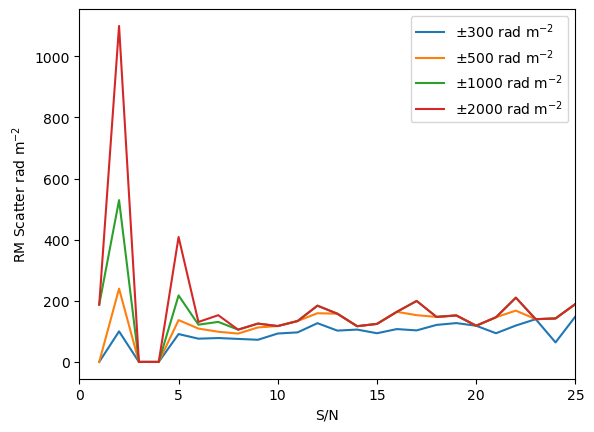
\includegraphics[width=\linewidth]{signal_to_noise.png}

        \caption[Rotation Measure scatter]{Plot showing scatter of RM as a function of signal to polarisation noise ratio for four Faraday depth search limits}
    \label{fig: s/n}
\end{figure}

With the signal-to-noise threshold found, I then created a rotation measure grid which showed the RM value found for each source with a signal to noise ratio above eight. The grid can be seen in Figure \ref{fig:1Grid} and shows a large variation across the field. The colour scale has been saturated at $\pm$ 400 rad$\,$m$^{\shortminus2}$ for ease of comparison with the Galactic latitude field in Figure \ref{fig: Shannon's RM grids}, however the RM values found range between a maximum of 696.8 rad$\,$m$^{\shortminus2}$ and a minimum of -697.3 rad$\,$m$^{\shortminus2}$. Within the Galactic plane the RM is mostly positive or zero however there are a few sources with a negative RM. This suggests that the magnetic field is being rotated clockwise as it passes through Faraday screen along the line of sight. These changes occur in over very short distances, so to get a better understanding of the scale of these changes I conducted a structure function analysis on the field. The density of RM sources can be seen to considerably decrease close to the bottom and left hand side of the field. This is due to the noisy edges contaminating these sources. This drop off in source density is not visible before the signal to noise ratio threshold is applied to the RM sources.



\begin{figure}
    \centering
    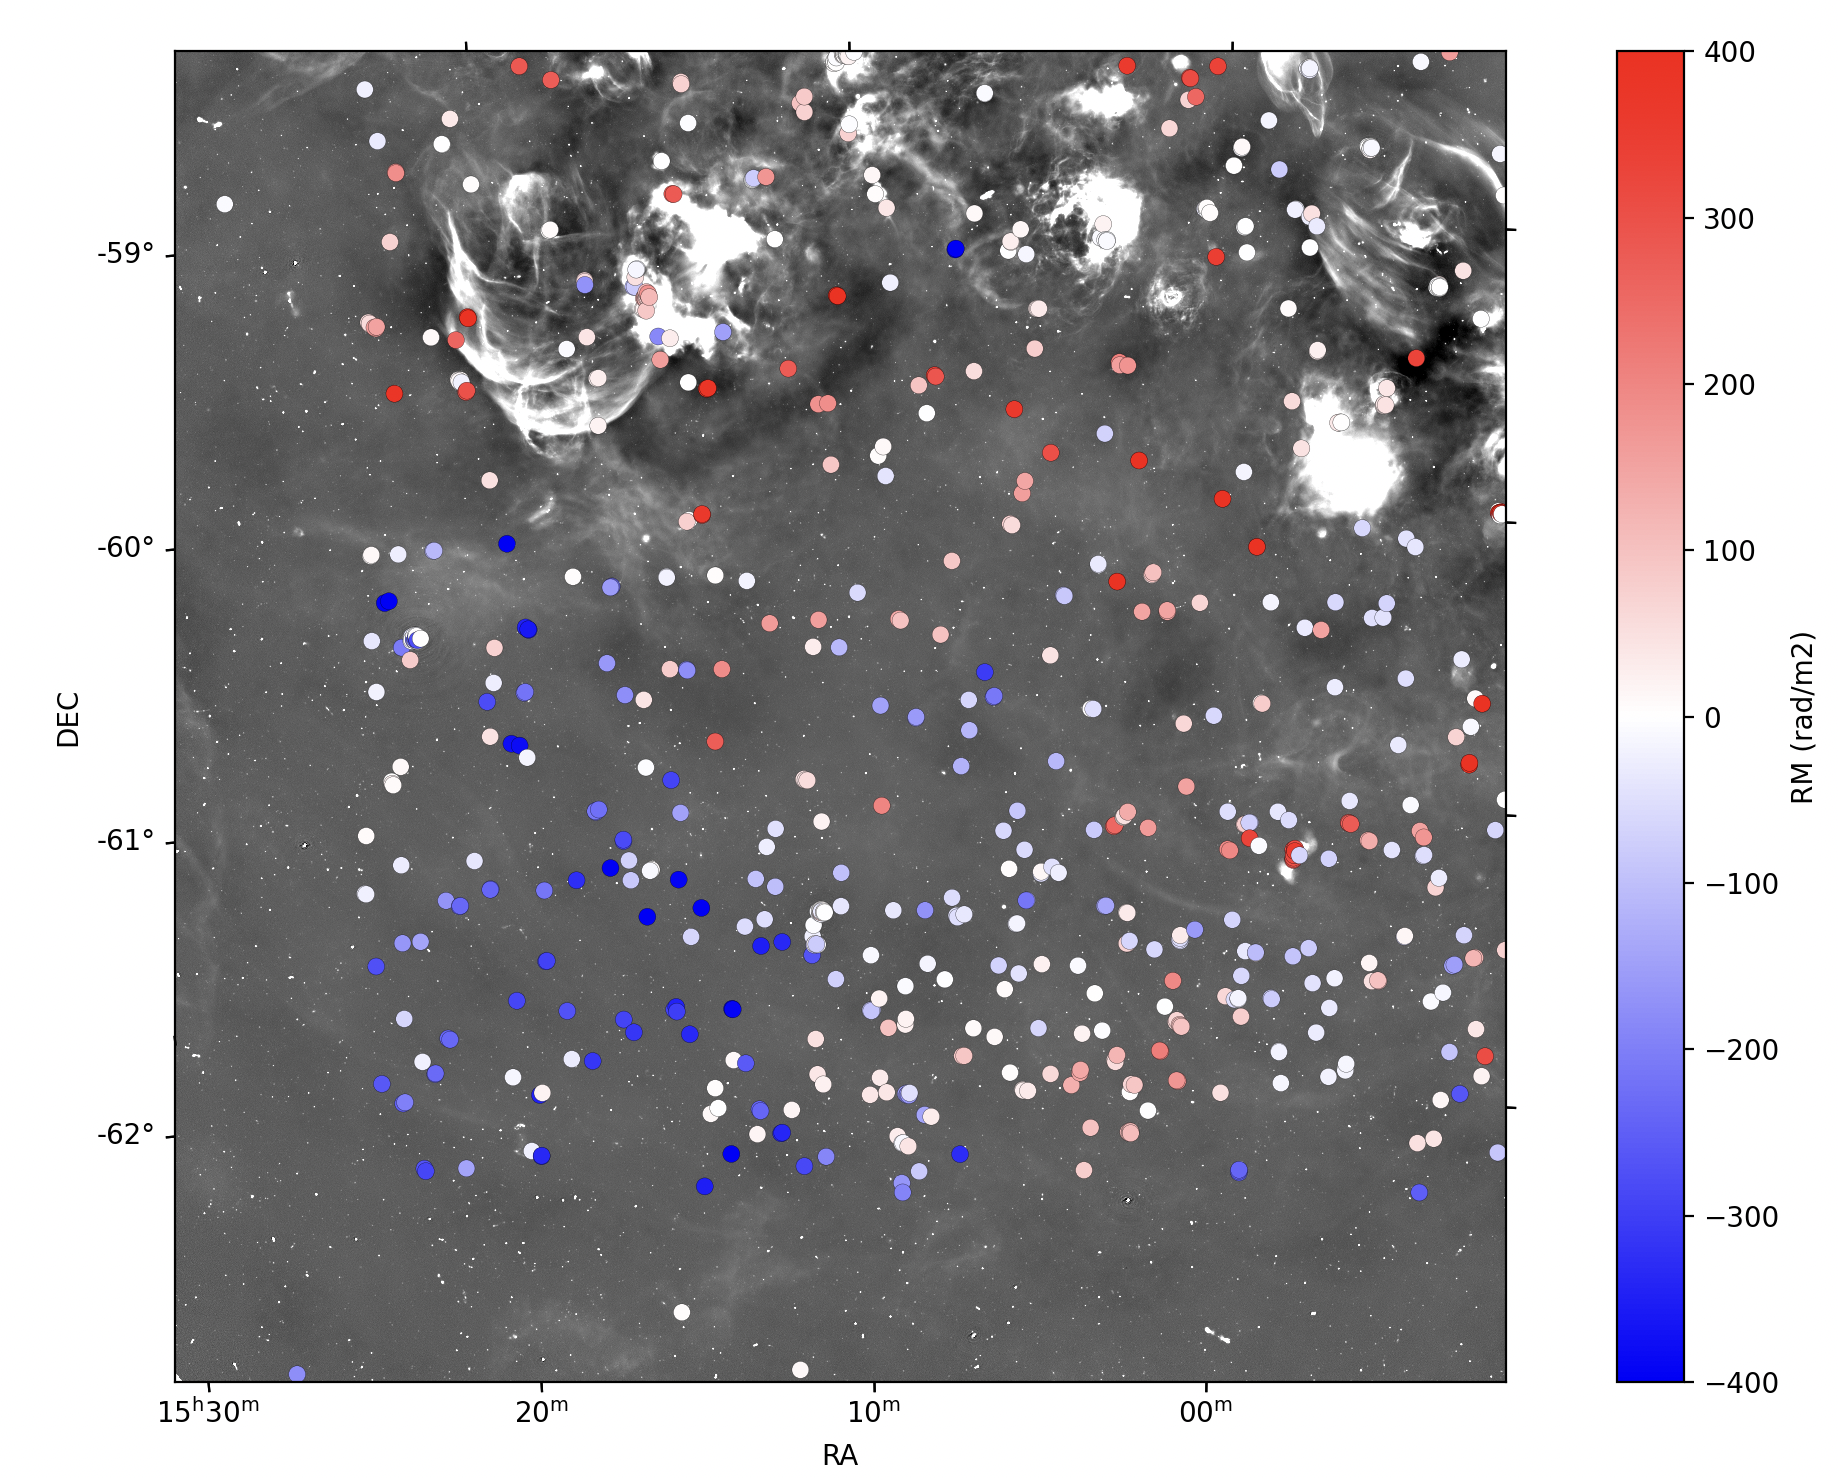
\includegraphics[width=\linewidth]{Thesis_Template/Figures/rm_without_nebulae.png}

        \caption[RM Grid]{RM grid showing the RM value for each source with a signal to noise ratio above 8, with red indicating a positive rotation measure and blue indicating a negative rotation measure. The colour scale is saturated at $\pm$ 400 rad$\,$m$^{\shortminus2}$}
    \label{fig:1Grid}
\end{figure}



\subsection{Structure Function Analysis}

Structure function analysis was performed in order to quantitatively understand the variation in RM across the field and the physical scale on which they occur.

The structure function equation gives a measure of the mean RM given a separation between two sources.

\begin{equation}
    STF(|\theta_i - \theta_j|) = \frac{1}{n}\underset{ij}{\Sigma}(RM(\theta_i) - RM(\theta_j))^2
    \label{Structure Function}
\end{equation}

\noindent where $\theta$ is the angular separation and $n$ is the number of sources in each bin (e.g. \cite{simonetti_1986}).

To apply this to the data I first removed any sources with a signal to noise ratio less than 8 from the catalogue, which left 823 sources. I next calculated the angular separation, $\theta$, and position angle between each pair of sources and created 18 bins between 0 and 360 arcseconds in angular separation and 6 bins between 0 and 180 arcseconds in position angle, where 0 is in the North-South direction. 

For each pair of sources I calculated the square of the differences and added it to the appropriate position bin. Finally I normalised the results by dividing by the number of pairs of sources in each bin, $n$. This is shown in Figure \ref{fig:2d_stf}. The lighter the structure function bin, the greater the variation of RM within the bin, so Figure \ref{fig:2d_stf} is showing that variation of RMs across the field varies most on scales of 300''-330'' angular separation and separations of 60''-90'' position angles.



\begin{figure}
        \centering
        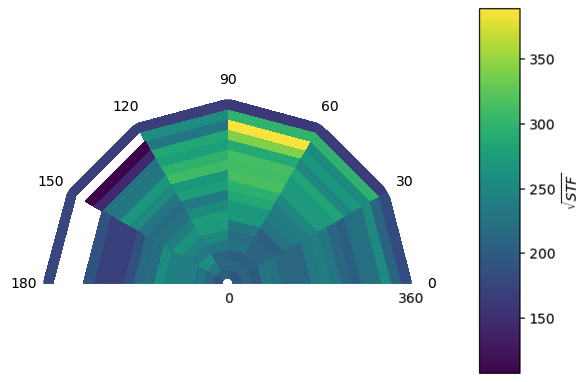
\includegraphics[width=\linewidth]{Thesis_Template/Figures/2D_STF.png}
        \caption[2D Structure Function]{2D structure function which shows the average rotation measure (in rad$\,$m$^{\shortminus2}$) given the separation between pairs of points in position angle and angular scale (both in arcseconds)}
        \label{fig:2d_stf}
    \end{figure}

In order to produce a one dimensional structure function, I then took the mean of all position angle bins for each separation angle bin, to produce Figure \ref{fig:1d_stf}.



\begin{figure}
        \centering
        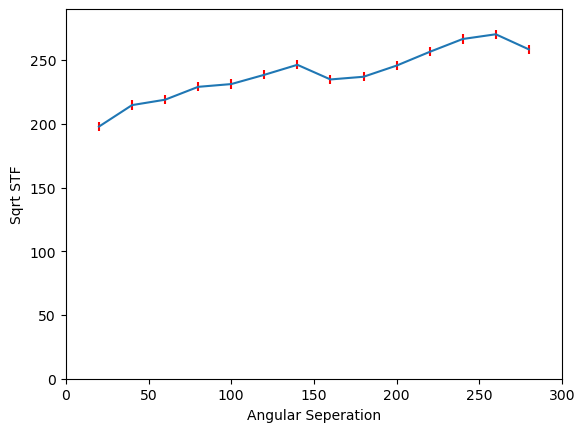
\includegraphics[width=\linewidth]{Thesis_Template/Figures/1D Structure Function.png}
        \caption[1D Structure Function]{1D structure function which shows the average rotation measure (in rad$\,$m$^{\shortminus2}$) as a function of angular separation (in arcseconds) between pairs of sources}
        \label{fig:1d_stf}
    \end{figure}

Both Figures \ref{fig:2d_stf} and \ref{fig:1d_stf}  show a general increasing trend of average rotation measure given two sources of increasing separation by both position angle and angular separation. The smaller difference, and blank sectors, seen towards the larger distance between sources in both position angle and angular separation in Figure \ref{fig:2d_stf} is due to very few, or no, pairs in those separation bins. Figure \ref{fig:2d_stf} shows a peak in the structure function in the position angle bin between $60^\circ$ and $90^\circ$, which is along the Galactic plane. This suggests that RM varies more along the plane than perpendicular to it. It is also interesting to note the steep rise to a high value for the structure function at such low separations, most clearly visible in Figure \ref{fig:1d_stf} but can also be seen in Figure \ref{fig:2d_stf}. This consistently high difference between RM at all separations suggests that there is rapidly varying small scale structure within the magnetic field of spiral arms. 

The field EMU1505-60 has a galactic longitude of approximately 319$^\circ$. Using the diagram of the Milky Way shown in Figure \ref{fig:mw map} to estimate distances, the line of sight first passes through the Sagittarius arm at a distance of approximately 1$\,$kpc, then the Scutum-Centaurus spiral arm twice at approximately 4$\,$kpc and 13$\,$kpc and finally the Sagittarius arm again at 17$\,$kpc. The emission and rotation from hte arms likely play a role in the variation seen in this RM grid.

\begin{figure}
    \centering
    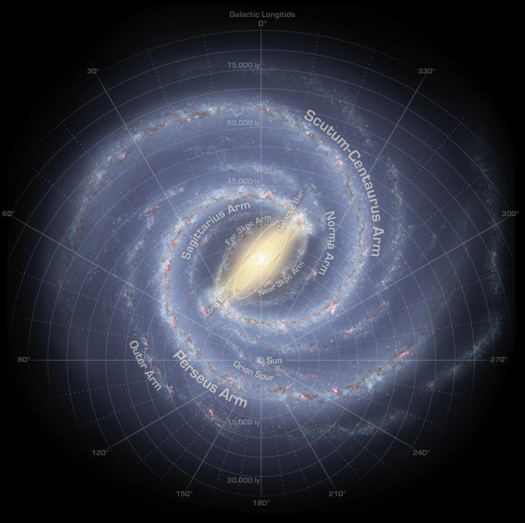
\includegraphics[width=\linewidth]{Thesis_Template/Figures/Milky Way Map.png}
    \caption[Diagram of the Milky Way]{Diagram of Milky Way with spiral arms and Galactic longitude labels, taken from \cite{spitzer_2009}}
    \label{fig:mw map}
\end{figure}

These angular scales correspond to variations of RM on scales of approximately 1$\,$pc at the first crossing of the Sagittarius arm, and 3$\shortminus$9$\,$pc at the two crossings of the Scutum-Centaurus spiral arm and 12$\,$pc variations at the second Sagittarius crossing. This result shows variation on a smaller scale than previous results which show variation on scales of $\sim$12$\shortminus$24$\,$pc at a distance of 1$\shortminus$2$\,$kpc (\cite{vanderwoude2024prototypefaradayrotationmeasure}, \cite{Haverkorn_2006}). This could suggest that this line of sight is more dominated by diffuse emission from the secondary passing of the Scutum-Centaurus band. Investigations of this over larger fields that will be possible when more fields from POSSUM are available will allow for a better understanding. 

%log plot to compare to vanderwoude and haverkorn?


